\pagebreak
\section{Timer}
Parte fondamentale per il funzionamento del microcontrollore è il Timer. In particolare, il timer è fondamentale per scandire il rateo delle operazioni della CPU e per dare un tempo di esecuzione alle periferiche.\\

Nel microcontrollore che abbiamo usato non c'è un singolo timer e ognuno ha caratteristiche, precisione e funzionalità diverse. 
Per i nostri scopi, noi abbiamo interagito con il Timer 6 che è un timer PLL

\subsection{Funzionamento}
I clock PLL (o phase locked loop) sono dei clock che sfruttano un clock di riferimento, nel nostro caso di quarzo, per generare un clock a frequenze più alte. Questo processo avviene attraverso un Voltage Control Oscillator il quale è in grado di generare onde quadre a frequenze molto alte e un Filtro passa Basso che fa da filtro per le armoniche generate dal VCO.\\

\begin{figure}[h]
    \centering
    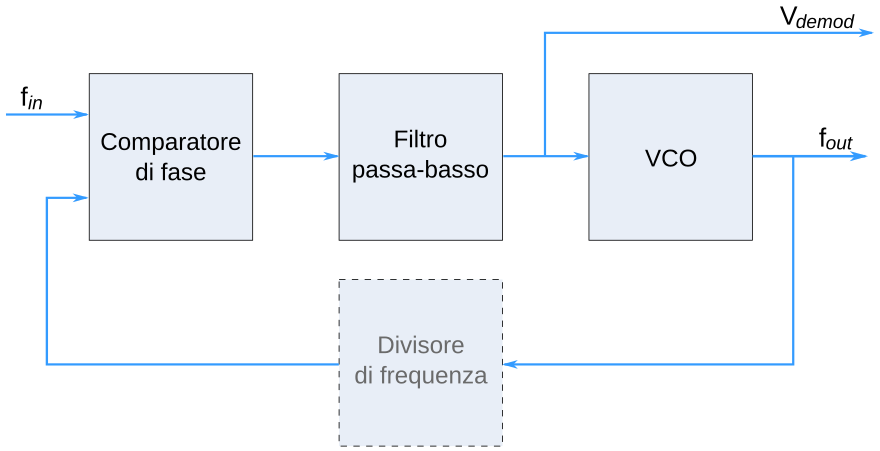
\includegraphics[width=0.7\linewidth]{microcontrollore/assets/PLL1_it.png}
    \caption{Schema di funzionamento del Timer}
    \label{fig:Timer}
\end{figure}

Questi 2 componenti, collegati ad un comparatore e al cristallo di riferimento riescono a generare onde quadre ad un ritmo costante usando il quarzo, molto stabile, come riferimento per non perdere la periodicità.\\
A questo processo si aggiungono altri componenti come il prescaler e il contatore che permettono di avere un controllo più preciso sulla frequenza del clock generato.\\

Per avere la massima velocità di esecuzione del programma, vanno modificate le frequenze dei clock. Così facendo, si possono velocizzare i processi più lenti a discapito di altri e di un maggior consumo di energia.\\

\subsection{Programmazione}
Per configurare il Timer 6, abbiamo usato STM32CubeMX. Questo programma permette di configurare ogni singolo timer a piacere, a patto di non uscire dai limiti del microcontrollore. Questo processo si fa attraverso un'interfaccia grafica dedicata

\begin{figure}
    \centering
    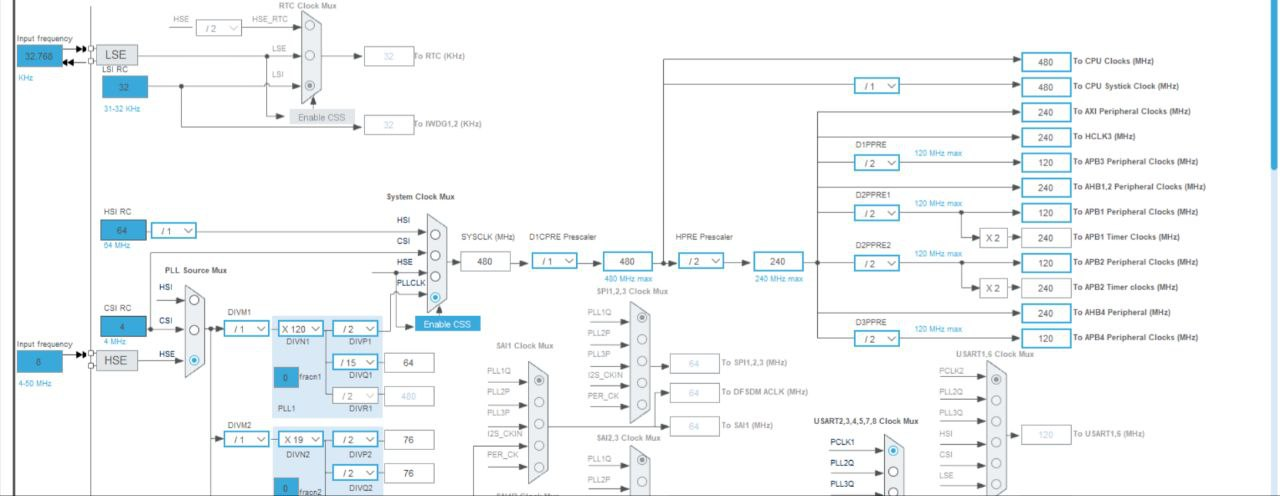
\includegraphics[width=0.7\linewidth]{microcontrollore/assets/clock_config.jpg}
    \caption{pagina di configurazione del clock all'interno di STM32CubeMX}
    \label{fig:Timer}
\end{figure}
 
Una volta configurato, si può passare all'inizializzazione del Timer.

\begin{minted}[bgcolor=coding , linenos]{C}
    void ESPE_TIM6_init(void){
        TIM6->CNT = 0; //Resetta il contatore
        TIM6->ARR = 10;//Setta il valore di auto reload
        TIM6->PSC = 24;//Setta il prescaler
    }
\end{minted}

Così facendo si può ulteriormente modificare la frequenza del timer e quindi la velocità delle periferiche ad essere collegate.\\
Per attivare il timer, si usa la funzione:
\begin{minted}[bgcolor=coding , linenos]{C}
    TIM6->CR1 |= TIM_CR1_CEN;
\end{minted}

Nel caso ce ne sia necessità il timer ha anche un interrupt che viene chiamato quando il contatore arriva al valore di auto reload, ma l'utilizzo del timer è stato quello di collegarlo all'ADC per far sì di avere misure equamente distanziate nel tempo, cosa non scontata a causa del metodo di conversione dell'ADC.\\